%experiments overview

\begin{frame}{KASCADE-Grande}
\begin{itemize}
  \item Proposed in 1989---disassembled in 2013;
  \item Aimed at studying
  high-evergy (galactic) cosmic rays by observing extensive air showers (EAS);
%   processes at the edge of the Galaxy and beyond by observing extended atmospheric showers (EAS);
  \item Consisted of:
  \begin{itemize}
    \item scintillators detecting $e$, $\gamma$, $\mu$:
    \begin{itemize}
  %сцинтиляторы, различают e, gamma, mu
    \item KASCADE---256 stations;
    \item GRANDE---37 stations;
    \end{itemize}
 %один большой калориметр
    \item Hadronic callorimeter;
 %радиодетектор
    \item Digital radio array LOPES detecting $e$, $e^{+}$;
% позволяющих наблюдать различные компоненты ливня
  \end{itemize}
  \item Important features of cosmic-ray spectrum have been obtained. The data analysis is ongoing;
%  благодаря данным с эксперимента было открыто много всего ополезного, при этом анлиз данных продолжается. новые статьи выходят
  \item KCDC (\textbf{K}ASCADE \textbf{C}osmic Ray \textbf{D}ata \textbf{C}enter, \textcolor{blue}{\texttt{http://kcdc.ikp.kit.edu}}) is a dedicated portal where all the data collected are available online. % At the moment
\end{itemize}

\begin{tikzpicture}[remember picture,overlay]
  \node[xshift=-12ex,yshift=-21ex] at (current page.north east){%
    
\includegraphics[width=0.3\textwidth]{pics/KCDC-Logo.png}
  };
\end{tikzpicture}
% \parbox[t][0pt]{0pt}{
%   \vspace{-0.63\textheight}
%   ~\hspace{0.68\textwidth}
\includegraphics[width=0.3\textwidth]{pics/KCDC-Logo.png}
% }
\end{frame}



\begin{frame}{TAIGA}
\footnotesize
\vspace{-1em}
\begin{itemize}
 \item Started in the mid 90s, is still operating and continiously enhancend
%  \item Currently consists of 4 detectors presented + TUNKA IACT is under construction;
\end{itemize}
\vspace{-2em}
\begin{minipage}[t]{0.31\textwidth}
  \begin{block}{\small Tunka-133}
    \parbox[c][0.20\textheight][t]{1\textwidth}{
      \centering
      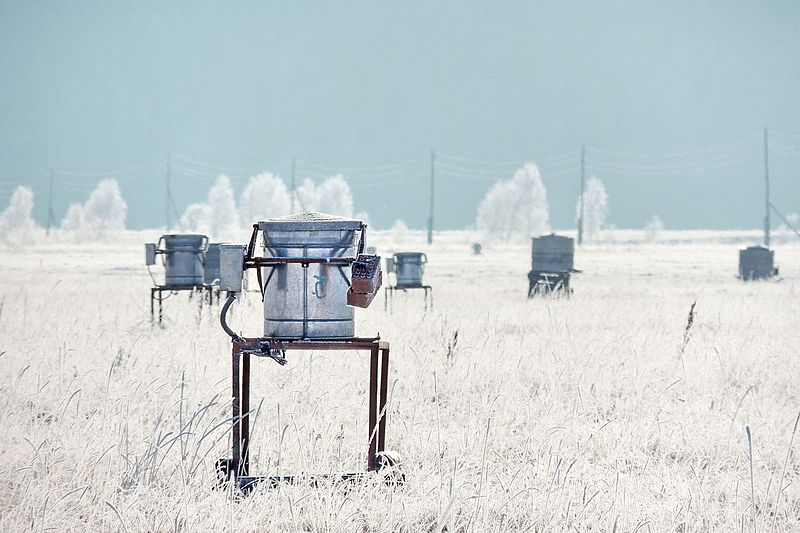
\includegraphics[width=0.7742\textwidth]{pics/Tunka-133.jpg}
    }
    \hfill
    \parbox[c][0.15\textheight][t]{1\textwidth}{
      \begin{itemize}
        \setlength{\itemsep}{0pt}
        \item 133 photomultipliers
        \item measures EAS Cherenkov light
      \end{itemize}
    }
  \end{block}
\end{minipage}
\hfill
\begin{minipage}[t]{0.31\textwidth}
  \begin{block}{\small Tunka-Rex}
    \parbox[c][0.20\textheight][t]{1\textwidth}{
      \centering
      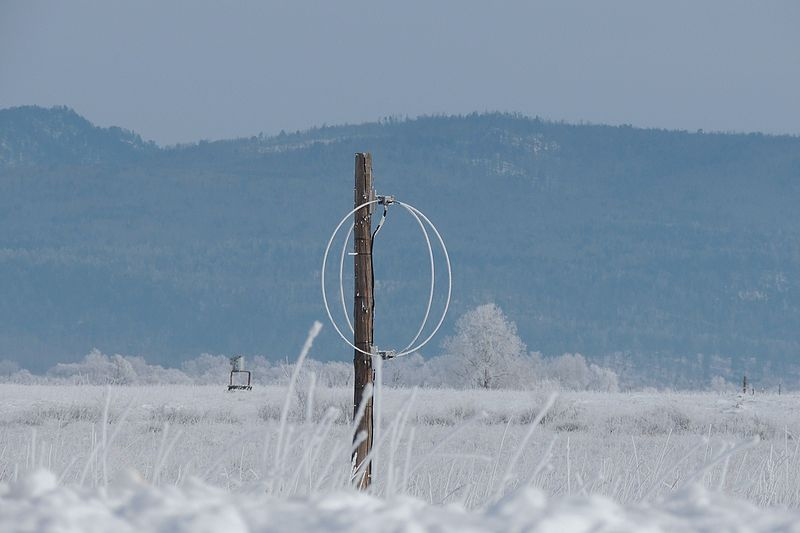
\includegraphics[width=0.7742\textwidth]{pics/Tunka-Rex.jpg}
    }
    \\
    \parbox[c][0.15\textheight][t]{1\textwidth}{
      \begin{itemize}
        \setlength{\itemsep}{0pt}
        \item 63 antennas
        \item measures EAS radio-emission
      \end{itemize}
    }
  \end{block}
\end{minipage}
\hfill
\begin{minipage}[t]{0.31\textwidth}
  \begin{block}{\small Tunka-HiSCORE}
    \parbox[c][0.20\textheight][t]{1\textwidth}{
      \centering
      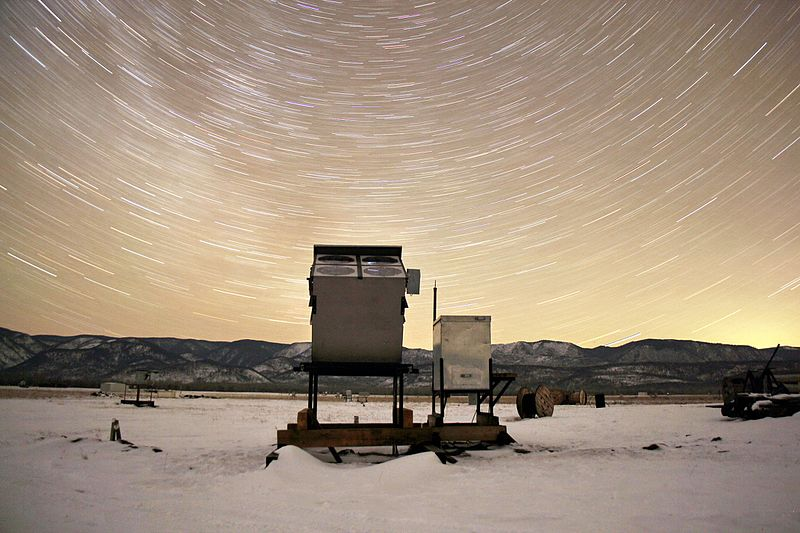
\includegraphics[width=0.7742\textwidth]{pics/Tunka-HiSCORE.jpg}
    }
    \\
    \parbox[c][0.15\textheight][t]{1.1\textwidth}{
      \begin{itemize}
        \setlength{\itemsep}{0pt}
        \item 47$\times$4 photomultipliers
        \item measures EAS Cherenkov light
      \end{itemize}
    }
  \end{block}
\end{minipage}

\vspace{-1ex}
\begin{minipage}[t]{0.48\textwidth}
  \begin{block}{\small Tunka-Grande}
    \parbox[c][0.21\textheight][t]{0.43\textwidth}{
      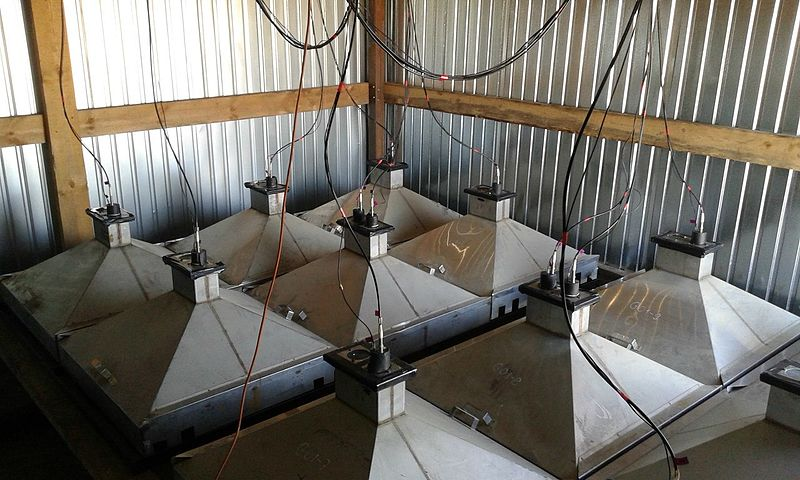
\includegraphics[width=0.50\textwidth]{pics/Hiller_Roman-005.jpg}
    }
    \hfill
    \parbox[c][0.21\textheight][t]{0.55\textwidth}{
      \begin{itemize}
        \setlength{\itemsep}{0pt}
        \item 380 scintillators 0.64m$^2$ each
        \item measures $e$/$\mu$ from EAS
      \end{itemize}
    }
  \end{block}
\end{minipage}
\hfill
\begin{minipage}[t]{0.48\textwidth}
  \begin{block}{\small Tunka-IACT}
    \parbox[c][0.21\textheight][t]{0.43\textwidth}{
      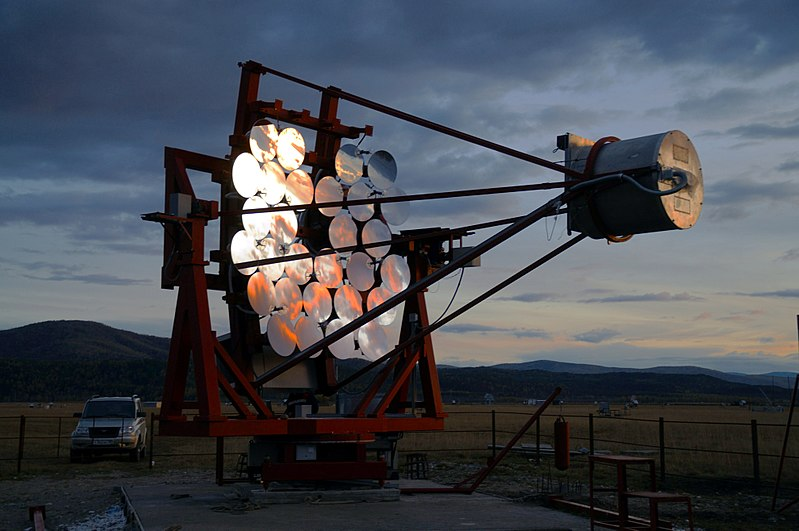
\includegraphics[width=0.50\textwidth]{pics/Tunka-Iact.jpg}
    }
    \hfill
    \parbox[c][0.21\textheight][t]{0.55\textwidth}{
      \begin{itemize}
        \setlength{\itemsep}{0pt}
        \item Imaging Air Cherenkov Telescopes
        \item is being extended
      \end{itemize}
    }
  \end{block}
\end{minipage}
\end{frame}

